\section{Introducción}
Ejemplo, es un documento anterior\\

\begin{Eq} [h!]
	\begin{equation}
		\hbar= 3.1416 . \frac{1}{3} \
	\end{equation}
	\caption{\textit{custom caption}}
\end{Eq}

\begin{equation}
	A+B = C_2\
\end{equation}

La enzima acetilcolinesterasa (AChE) desempeña un papel fundamental en la regulación de la transmisión del impulso nervioso en el sistema nervioso central y periférico. Su función principal radica en la hidrólisis del neurotransmisor acetilcolina, una molécula clave en la comunicación entre las células nerviosas. La acción de la AChE asegura la terminación precisa de las señales nerviosas, permitiendo una respuesta neuronal adecuada.\cite{soreq2001acetylcholinesterase}\\

La acetilcolina es liberada en las sinapsis neuronales y se une a los receptores de acetilcolina presentes en las células postsinápticas, transmitiendo la señal eléctrica de una neurona a otra. Una vez que la acetilcolina ha cumplido su función, la AChE entra en acción para hidrolizarla en colina y acetato. Esta reacción es esencial para eliminar la acetilcolina de la sinapsis y prevenir su acumulación excesiva, lo que podría interferir con la comunicación neuronal normal.\cite{massoulie1993structure}\\


\begin{figure}[h]
	\centering
	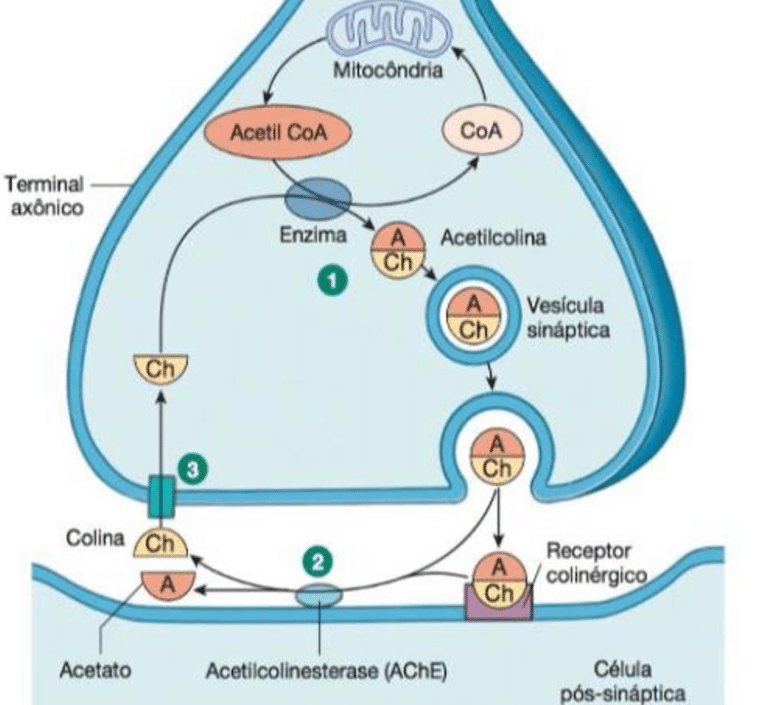
\includegraphics[width=2in]{img/f1.png}
	\caption{Metabolismo de la acetilcolina (ACh). La enzima acetilcolinesterasa descompone rápidamente la ACh en la sinapsis}
	\label{1}
\end{figure}

La inhibición de la acetilcolinesterasa tiene importantes implicaciones en la fisiología y la toxicología, ya que puede alterar la función normal del sistema nervioso y dar lugar a una serie de efectos adversos. Algunos compuestos, tanto naturales como sintéticos, pueden actuar como inhibidores de la AChE y afectar su actividad, lo que puede tener consecuencias graves para la salud humana y/o animal. \cite{nogueira2015toxicology}\\

Es importante destacar que los inhibidores de la AChE no solo pueden provenir de fuentes exógenas, como ciertos productos químicos y venenos de origen natural, sino que también pueden producirse endógenamente en condiciones patológicas. La inhibición de la AChE puede ser utilizada terapéuticamente en ciertos trastornos, como la enfermedad de Alzheimer, donde se busca aumentar la disponibilidad de acetilcolina en el cerebro. \cite{bartels2010parkinson}\\

En este informe, nos centraremos en la importancia de la reacción de inhibición de la acetilcolinesterasa por el Malathion, un insecticida ampliamente utilizado en el mundo. \cite{Geed2016}


\section{Malathion}

El malathion, un líquido con olor a zorrillo o ajo, es un insecticida organofosforado de amplio espectro  utilizado en la agricultura  y el control de plagas. Fue introducido por primera vez en los Estados Unidos en 1956 y está regulado por la Agencia de Protección Ambiental de los Estados Unidos (EPA).\\
Es posible encontrar este producto en el mercado hoy en día para uso comercial y doméstico a pesar de los hallazgos de que este y pesticidas similares son probablemente carcinógenos. Es considerablemente más seguro de usar que el \textit{paratión} organofosforado similar, que ha sido prohibido o restringido en todo el mundo.\cite{ACS} \\

\begin{figure}[h]
	\centering
	
\includegraphics[width=1.5in]{img/f2.png}
	\caption{Estructura Malathion.}
	\label{2}
\end{figure}


Actúa como un inhibidor irreversible de la AChE, lo que provoca la acumulación de acetilcolina en las sinapsis neuronales. A pesar de su potencial toxicidad, el Malathion ha sido evaluado y se ha determinado que su uso seguro es posible en humanos bajo condiciones adecuadas de aplicación y exposición controlada.\cite{Geed2016} \\

Además del Malathion, existen otros compuestos que también actúan como inhibidores de la AChE. Uno de ellos es el veneno de la mamba negra, una serpiente venenosa que se encuentra principalmente en África. El veneno de la mamba negra contiene neurotoxinas altamente potentes, como las dendrotoxinas, que tienen efectos directos y perjudiciales sobre el sistema nervioso humano.\cite{klaassen2018casarett}\\

\section{Mecanismo}

El modelo de Michaelis-Menten es una representación matemática de las reacciones enzimáticas, que describe la velocidad de la reacción en función de la concentración de sustrato y la eficiencia de la enzima. Según este modelo, la reacción enzimática entre la enzima (E) y el sustrato (S) forma un complejo enzima-sustrato (ES) reversible, que posteriormente se descompone en productos (P).\\

En el caso del malathion y la acetilcolinesterasa (AChE), el malathion (I) actúa como un sustrato para la enzima. Cuando el malatión está presente en el entorno de la enzima, se une al sitio activo de la enzima, formando un complejo enzima-inhibidor (EI).\\
Una vez que el malatión se une a la enzima, inhibe de manera irreversible su actividad catalítica. Esto significa que la enzima ya no puede llevar a cabo su función normal de hidrolizar la acetilcolina. La inhibición de la enzima resulta en la acumulación de acetilcolina en las sinapsis nerviosas, lo que provoca una interrupción en la transmisión de señales nerviosas y la parálisis de los insectos y otros organismos objetivo.\cite{Geed2016}\\

\begin{Eq} [h!]
	\begin{equation}
		\ce{E + ACh <=>[{k1}][{k_{-1}}] ACh-E ->[kcat] E + Act + Col}\\
	\end{equation}
	\caption{\textit{Hidrólisis de Acetilcolina (ACh)}}
\end{Eq}

\begin{Eq} [h!]
	\begin{equation}
		\ce{E + I ->[ki] EI}
	\end{equation}
	\caption{\textit{Reacción Enzima + Inhibidor, en este caso, inhibición de la Enzima Acetilcolinesterasa (AChE) }}
\end{Eq}

A continuación se muestra el mecanismo cinético de la enzima Acetilcolinesterasa con su sustrato Acetilcolina y con el Malathion.\\

Donde:\\

E.	Enzima Acetilcolinesterasa (AChE).\\
ACh.	Sustrato Acetilcolina.\\
ACh-E.	Complejo Enzima-Sustrato.\\
Act.	Acetil.\\
Col.	Colina.\\
I.	Malathion (inhibidor).\\
EI. Complejo Enzima-Inhibidor.\\

En este caso es una reacción simultánea donde la enzima tiene la misma probabilidad de reaccionar con el sustrato como con el inhibidor.

\section{Simulación}
Las reacciones cinéticas de este sistema se simulan mediante un código de Python, \href{https://colab.research.google.com/drive/1STolipp3le7wWiyVhjlUpjwr8-pAcXaQ?usp=sharing}{con el cual se puede interactuar desde este enlace.}\\
Las ecuaciones diferenciales que las modelan se presentan de la siguiente manera:\\

\begin{equation}
	v= \frac{dE}{dt} = -k1[E][ACh] + k_{-1}[ACh-E] + kcat [ACh-E] - ki [E] [I]
\end{equation}

\begin{equation}
	v= \frac{dACh}{dt} = -k1[E][ACh] + k_{-1}[ACh-E]
\end{equation}

\begin{equation}
	v= \frac{dACh-E}{dt} = k1[E][ACh] - k_{-1}[ACh-E] -kcat[ACh-E]
\end{equation}

\begin{equation}
	v= \frac{dAct}{dt} = kcat[ACh-E]
\end{equation}

\begin{equation}
	v= \frac{dCol}{dt} = kcat[ACh-E]
\end{equation}

\begin{equation}
	v= \frac{dI}{dt} = -ki[E][I]
\end{equation}

\begin{equation}
	v= \frac{dE-I}{dt} = ki[E][I]
\end{equation}

Con las ecuaciones y los siguientes parámetros se logró realizar la simulación.

\begin{table}[h]
	\centering
	\begin{tabular}{|c|c|}
		\hline
		\textbf{Concentración Inicial} & \textbf{Valor} \\
		\hline
		$E_0$                          & 1.0 mmol       \\
		\hline
		$ACh_0$                        & 1.5 mmol       \\
		\hline
		$I_0$                          & 0.8 mmol       \\
		\hline
	\end{tabular}
	\caption{Concentraciones Iniciales}
	\label{tab:concentraciones}
\end{table}

\begin{table}[h]
	\centering
	\begin{tabular}{|c|c|}
		\hline
		\textbf{Constante} & \textbf{Valor}         \\
		\hline
		$k_1$              & 0.02 $mol^{-1} s^{-1}$ \\
		\hline
		$k_{-1}$           & 0.015 $s^{-1}$         \\
		\hline
		$k_{\text{cat}}$   & 0.03 $s^{-1}$          \\
		\hline
		$k_i$              & 1.0 $mol^{-1} s^{-1}$  \\
		\hline
	\end{tabular}
	\caption{Constantes de velocidad}
	\label{tab:constantes}
\end{table}

\section{Resultados}

Se realizó la simulación de la hidrolisis de Acetilcolina, es decir, como funciona normalmente sin inhibidor. (\textit{ver Ec. 1.})

\begin{figure}[h]
	\centering
	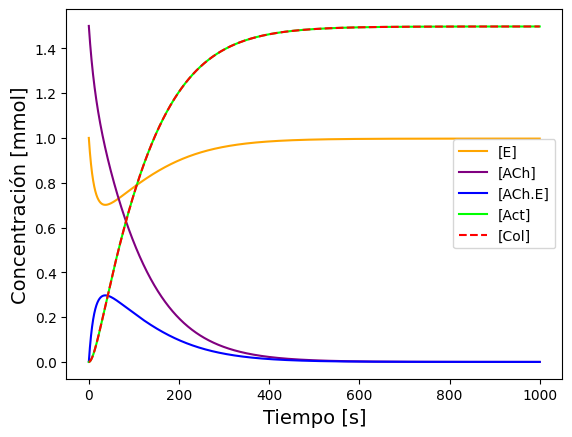
\includegraphics[width=\columnwidth]{img/simu_no_i.png}
	\caption{Hidrólisis ACh por la enzima AChE.}
	\label{3}
\end{figure}

Posterior se realizó la simulación con los mismos parámetros, añadiendo ahora el inhibidor.\\

\begin{figure}[h]
	\centering
	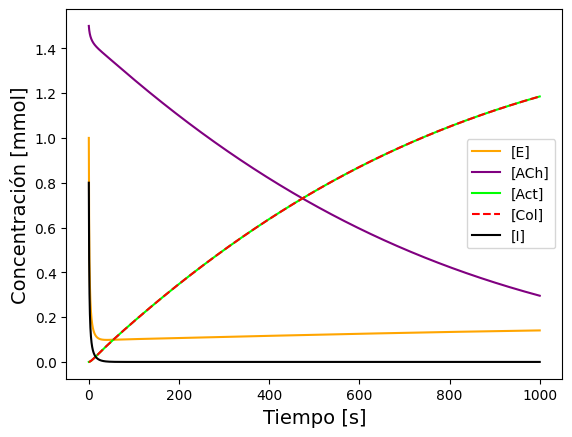
\includegraphics[width=\columnwidth]{img/simu_con_i.png}
	\caption{Inhibición de AChE por Malathion.}
	\label{4}
\end{figure}

Como se observa en la Figura 4, comienza una reacción competitiva entre el sustrato y el inhibidor por adherirse al sitio activo de la enzima. Se observa una disminución de la concentración de los productos.\\

\begin{figure}[h]
	\centering
	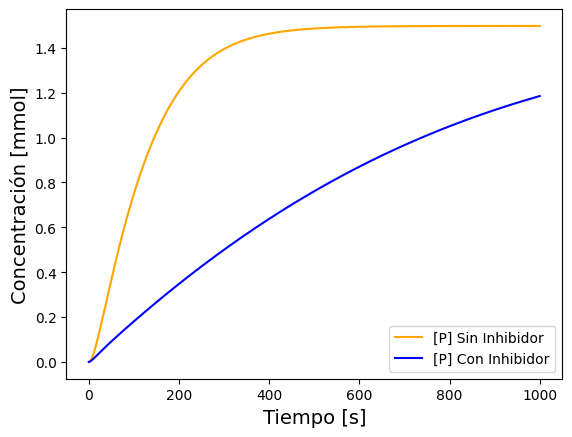
\includegraphics[width=\columnwidth]{img/simucomp.png}
	\caption{Formación de productos con y sin inhibidor. [Act] = [Col], por lo tanto [P] se refiere a la concentración de ambos productos.}
	\label{5}
\end{figure}

Se realizan cambios en la concentración del Malathion [I] y en el tiempo de reacción, respectivamente y dejando las demas variables constantes.\\

Al aumentar la concentración de [I] de 0.8 a 1.0 mmol se observa el comportamiento de la Figura 6.

\begin{figure}[h]
	\centering
	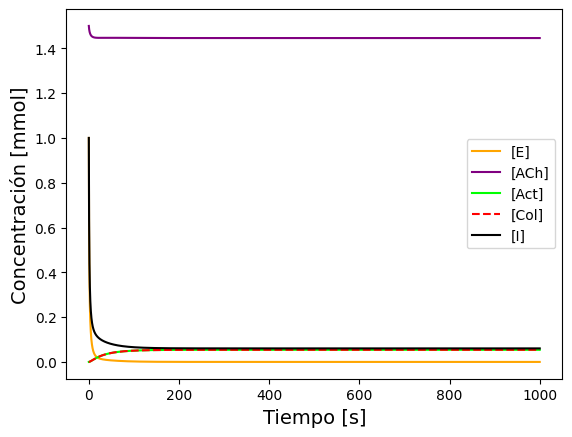
\includegraphics[width=\columnwidth]{img/masconc.png}
	\caption{Aumento de [I].}
	\label{6}
\end{figure}

Finalmente se aumento el parámetro del tiempo transcurrido, nuevamente dejando las demás variables constantes.

\begin{figure}[h]
	\centering
	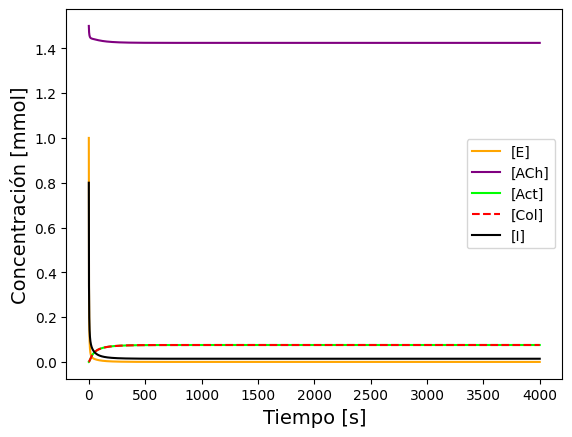
\includegraphics[width=\columnwidth]{img/mast.png}
	\caption{Aumento del tiempo de reacción.}
	\label{7}
\end{figure}

\section{Análisis y Conclusiones}

Se observa una clara diferencia entre la reacción sin inhibidor y la que sí lo tiene, el descenso de la concentración de los productos depende de la concentración del inhibidor(Malathion), pues compite con la mayor concentración de sustrato(ACh) en el medio y ambas tienen la misma probabilidad de fijarse a la enzima(AChE), la diferencia es que el inhibidor realiza una reacción irreversible con la enzima, lo que disminuye la cantidad de enzimas disponibles,caso opuesto, cuando el complejo enzima-sustrato hidroliza el \textit{ACh}, queda libre nuevamente para reaccionar ya sea con el inhibidor o con el sustrato. En la Figura 5 se observa como vuelve a subir la [E] debido a la reacción y que no hay inhibidor, en la Figura 6 la [E] no vuelve a subir debido a la reacción irrversible de \textit{E + I}. \\

Con respecto al aumento de concentración del Malathion, aunque el sustrato tiene un 50\% más de concentración que el inhibidor, resulta altamente efectiva la inhibición de la enzima, pues aumenta la probabilidad de la adhesión \textit{E-I}.

Cuando aumenta el tiempo, también la inhibición pues al ser una reacción irreversible la enzima con el inhibidor no vuelve a liberarse la enzima y con el paso del tiempo habrá menos enzimas.


El malathion es un insecticida muy efectivo, pues con poca concentración es posible terminar con las plagas de insectos principalmente, ya se estudió el mecanismo de acción del malathion, la acetilcolina se acumula en las sinapsis nerviosas del insecto, causando una sobreestimulación de los receptores de acetilcolina y una interrupción en la transmisión de señales nerviosas. Esto lleva a la parálisis y muerte del insecto.

\bibliographystyle{plain}
\bibliography{lib/biblio}